\section{Secondary Chilled Water Loop -- Plate Heat Exchanger}\label{secondary-chilled-water-loop-plate-heat-exchanger}

The Secondary Cooling system is constructed by using a \emph{PlantLoop} object, the working fluid in this loop is water. It uses one side of a plate heat exchanger (modeled using a \emph{HeatExchanger:FluidToFluid} object) to supply chilled water to a cooling coil (modeled by using a \emph{Coil:Cooling:DetailedGeometry} object). Therefore, the supply side of the loop contains the heat exchanger and the demand side contains the cooling coil. The loop is operated by using plant equipment operation schemes, and schedules. ~Refer to Figure~\ref{fig:simple-line-diagram-for-the-secondary-chilled} for a simple diagram of the secondary chilled water loop.

\begin{figure}[hbtp] % fig 103
\centering
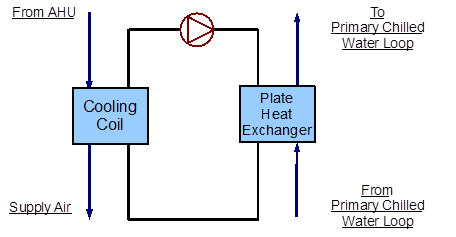
\includegraphics[width=0.9\textwidth, height=0.9\textheight, keepaspectratio=true]{media/image103.png}
\caption{Simple line diagram for the secondary chilled water loop \protect \label{fig:simple-line-diagram-for-the-secondary-chilled}}
\end{figure}

\subsection{Flowcharts for the Secondary Chilled Water Loop Input Process}\label{flowcharts-for-the-secondary-chilled-water-loop-input-process}

This series of flowcharts serve as a guide for identifying and inputting the secondary chilled water loop and its components into the input file. The EnergyPlus line diagram for this loop is provided in Figure~\ref{fig:energyplus-line-diagram-for-the-secondary}. A simple flowchart for the separation of the half loops is provided in Figure~\ref{fig:simple-flow-chart-for-separation-on-half-003}.

\begin{figure}[hbtp] % fig 104
\centering

\includegraphics[width=0.9\textwidth, height=0.9\textheight, keepaspectratio=true]{media/image104.png}
\caption{EnergyPlus line diagram for the secondary chilled water loop \protect \label{fig:energyplus-line-diagram-for-the-secondary}}
\end{figure}

\begin{figure}[hbtp] % fig 105
\centering
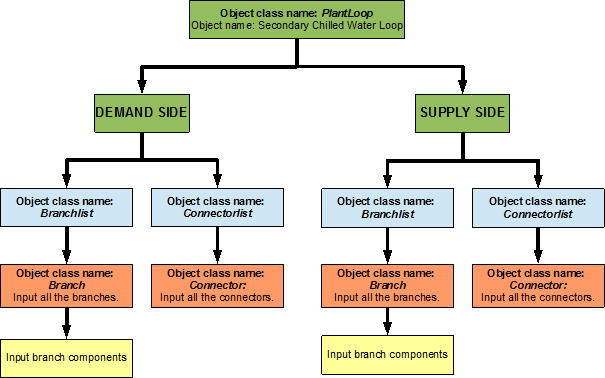
\includegraphics[width=0.9\textwidth, height=0.9\textheight, keepaspectratio=true]{media/image105.png}
\caption{Simple flow chart for separation on half loops in the secondary chilled water loop \protect \label{fig:simple-flow-chart-for-separation-on-half-003}}
\end{figure}

\subsubsection{Secondary Chilled Water Loop Supply Side Loop Construction}\label{secondary-chilled-water-loop-supply-side-loop-construction}

The main components on the supply side half loop for the Secondary Cooling System are the plate heat exchanger that supplies the chilled water and the variable speed pump that circulates the chilled water through the loop. The variable speed pump (named `CW Sec Circ Pump') is the secondary pump in the primary/secondary pumping setup. This half loop supplies chilled water to a cooling coil on the demand side half loop. The supply side half loop contains four components, four branches, eight nodes, and one splitter-mixer pair. The EnergyPlus line diagram for the secondary chilled water loop supply side is provided in Figure~\ref{fig:energyplus-line-diagram-for-the-supply-side-007}. The flowchart for supply side branches and components is provided in Figure~\ref{fig:flowchart-for-secondary-chilled-water-loop-supply-side-007}. The flowchart for supply side connectors is provided in Figure~\ref{fig:flowchart-for-secondary-chilled-water-loop-supply-side-connectors}.

\begin{figure}[hbtp] % fig 106
\centering
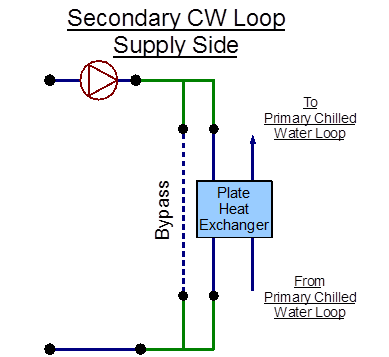
\includegraphics[width=0.9\textwidth, height=0.9\textheight, keepaspectratio=true]{media/image106.png}
\caption{EnergyPlus line diagram for the supply side of the secondary chilled water loop \protect \label{fig:energyplus-line-diagram-for-the-supply-side-007}}
\end{figure}

\begin{figure}[hbtp] % fig 107
\centering
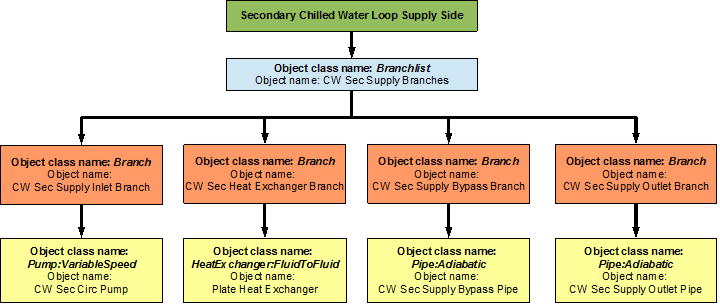
\includegraphics[width=0.9\textwidth, height=0.9\textheight, keepaspectratio=true]{media/image107.png}
\caption{Flowchart for secondary chilled water loop supply side branches and components \protect \label{fig:flowchart-for-secondary-chilled-water-loop-supply-side-007}}
\end{figure}

\begin{figure}[hbtp] % fig 108
\centering

\includegraphics[width=0.9\textwidth, height=0.9\textheight, keepaspectratio=true]{media/image108.png}
\caption{Flowchart for secondary chilled water loop supply side connectors \protect \label{fig:flowchart-for-secondary-chilled-water-loop-supply-side-connectors}}
\end{figure}

\subsubsection{Secondary Chilled Water Loop Demand Side Loop Construction}\label{secondary-chilled-water-loop-demand-side-loop-construction}

The main component on the demand side half loop is the Cooling Coil that cools the air in the building by using the chilled water that is supplied by the plate heat exchanger. This side of the loop also has eight nodes, four components, four branches, and one splitter-mixer pair. An EnergyPlus schematic for the demand side is provided in Figure~\ref{fig:energyplus-line-diagram-for-the-demand-side-007}. The flowchart for demand side branch definition is provided in Figure~\ref{fig:flowchart-for-secondary-chilled-water-loop-demand-side-007}. The flowchart for the demand side connectors is provided in Figure~\ref{fig:flowchart-for-secondary-chilled-water-loop-demand-side-connectors}.

\begin{figure}[hbtp] % fig 109
\centering
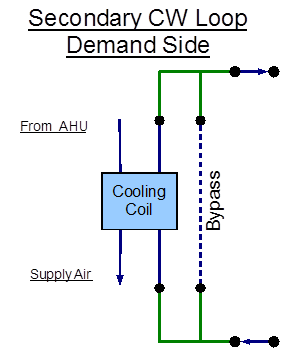
\includegraphics[width=0.9\textwidth, height=0.9\textheight, keepaspectratio=true]{media/image109.png}
\caption{EnergyPlus line diagram for the demand side of the secondary chilled water loop \protect \label{fig:energyplus-line-diagram-for-the-demand-side-007}}
\end{figure}

\begin{figure}[hbtp] % fig 110
\centering
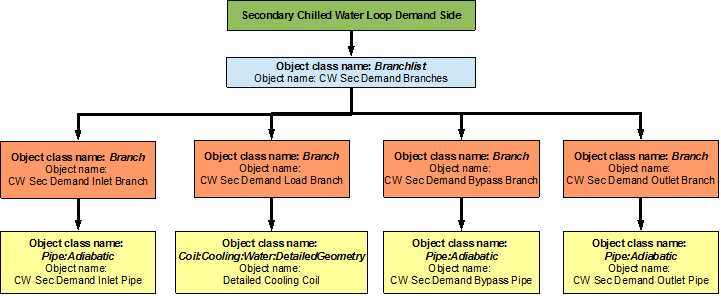
\includegraphics[width=0.9\textwidth, height=0.9\textheight, keepaspectratio=true]{media/image110.png}
\caption{Flowchart for secondary chilled water loop demand side branches and components \protect \label{fig:flowchart-for-secondary-chilled-water-loop-demand-side-007}}
\end{figure}

\begin{figure}[hbtp] % fig 111
\centering

\includegraphics[width=0.9\textwidth, height=0.9\textheight, keepaspectratio=true]{media/image111.png}
\caption{Flowchart for secondary chilled water loop demand side connectors \protect \label{fig:flowchart-for-secondary-chilled-water-loop-demand-side-connectors}}
\end{figure}

\subsection{Flowcharts for secondary chilled water loop Controls}\label{flowcharts-for-secondary-chilled-water-loop-controls}

The secondary chilled water loop is operated by using set-points, plant equipment operation schemes and schedules.

\subsubsection{Secondary Chilled Water Loop Schedules}\label{secondary-chilled-water-loop-schedules}

The flowchart for Primary Cooling loop schedule definition is provided in Figure~\ref{fig:flowchart-for-secondary-chilled-water-loop-schedules}. The Secondary Cooling loop uses two different schedules to operate properly. \emph{ON} is a compact schedule that keeps the plate heat exchanger running at all times of the day, this compact schedule uses a continuous \emph{ScheduleTypeLimit} (\emph{Fraction)} which defines that the value of On is 1 and that of Off is 0. This plant loop also uses another compact schedule named \emph{CW Sec Loop Temp Schedule} declares that the outlet temperature of the Secondary Cooling loop should be 6.67 degrees Celsius at any time; this schedule is used by the setpoint manager (\emph{CW Sec Loop Setpoint Manager)}. This schedule uses a schedule type limit named \emph{Temperature,} which defines the loop upper and lower temperature limits.

\begin{figure}[hbtp] % fig 112
\centering

\includegraphics[width=0.9\textwidth, height=0.9\textheight, keepaspectratio=true]{media/image112.png}
\caption{Flowchart for secondary chilled water loop schedules \protect \label{fig:flowchart-for-secondary-chilled-water-loop-schedules}}
\end{figure}

\subsubsection{Secondary Chilled Water Loop Plant Equipment Operation Schemes}\label{secondary-chilled-water-loop-plant-equipment-operation-schemes}

The \emph{PlantEquipmentOperationschemes} object uses the \emph{ON} schedule and the \emph{CW Sec Operation Scheme} objects to set the range of the demand loads for which the heat exchanger is operated during the simulation period. A flowchart detailing the secondary chilled water loop plant equipment operation schemes is provided in Figure~\ref{fig:flowchart-for-secondary-chilled-water-loop-plant-equipment-operation}.

\begin{figure}[hbtp] % fig 113
\centering

\includegraphics[width=0.9\textwidth, height=0.9\textheight, keepaspectratio=true]{media/image113.png}
\caption{Flowchart for secondary chilled water loop plant equipment operation schemes \protect \label{fig:flowchart-for-secondary-chilled-water-loop-plant-equipment-operation}}
\end{figure}

\subsubsection{Secondary Chilled Water Loop Setpoints}\label{secondary-chilled-water-loop-setpoints}

The \emph{CW Sec Loop Setpoint Manager} uses the \emph{CW Sec Loop Temp Schedule} to set a temperature control point at the \emph{CW Sec Supply Outlet Node}. This setpoint allows the program to control the temperature at the node by operating the components in the Secondary Cooling loop. A flowchart for Secondary Cooling loop setpoints is provided in Figure~\ref{fig:flowchart-for-secondary-chilled-water-loop-setpoints}.

\begin{figure}[hbtp] % fig 114
\centering

\includegraphics[width=0.9\textwidth, height=0.9\textheight, keepaspectratio=true]{media/image114.png}
\caption{Flowchart for secondary chilled water loop setpoints \protect \label{fig:flowchart-for-secondary-chilled-water-loop-setpoints}}
\end{figure}

\subsubsection{Secondary Chilled Water Loop Sizing}\label{secondary-chilled-water-loop-sizing}

The secondary chilled water loop is sized such a way that the design loop exit temperature is 6.67 degrees Celsius, and the loop design temperature difference is 5 degrees Celsius. A flowchart for the chilled water loop sizing is provided in Figure~\ref{fig:flowchart-for-secondary-chilled-water-loop-sizing}.

\begin{figure}[hbtp] % fig 115
\centering
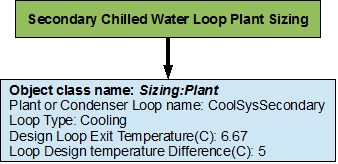
\includegraphics[width=0.9\textwidth, height=0.9\textheight, keepaspectratio=true]{media/image115.png}
\caption{Flowchart for secondary chilled water loop sizing \protect \label{fig:flowchart-for-secondary-chilled-water-loop-sizing}}
\end{figure}
